\documentclass[12pt,a4paper]{article}
\usepackage{geometry}
\usepackage[numbers]{natbib}
\usepackage{amssymb, amsmath}
\usepackage{graphicx}
\usepackage{grffile}
\graphicspath{{../Figures/}}
\usepackage{gensymb}
\usepackage[font=small]{caption}
\usepackage[utf8]{inputenc}
\usepackage[english]{babel}
\usepackage{fancyhdr}
\usepackage[raggedright]{titlesec}
\usepackage{subcaption}
\usepackage{multirow}
\usepackage{dirtytalk}
\usepackage{framed}
\usepackage[normalem]{ulem}
\usepackage[pdftex,breaklinks]{hyperref}
\hypersetup{
  colorlinks   = true, %Colours links instead of ugly boxes
  urlcolor     = green, %Colour for external hyperlinks
  linkcolor    = blue, %Colour of internal links
  citecolor   = red %Colour of citations
}


\begin{document}
\author{Katrina Ashton}


\pagestyle{fancy}
\fancyhf{}
\rhead{\thepage}
\lhead{u5586882}

\section{What I've done}
\begin{itemize}
\item{Modified code to capture the depth image associated with each RGB image and point cloud}
\item{Had a look into the Vicon code}
\item{Covered cube box in pictures to add texture}
\item{Collected more data (checkered box and cube box as scene), didn't manage to get a full run without crashing though. It got about halfway around the boxes both times.}
%\item{Added more to the appendices for the final report draft}
\end{itemize}

\section{Parts of report to look at}
\begin{itemize}
\item{Nothing new.}
\end{itemize}

\section{Questions}
\begin{itemize}
\item
\end{itemize}

\section{Comments}
\begin{itemize}
\item The quadcopter is actually publishing its commands, so I'm recording a rosbag of that topic now
\item The top box is not really in the image being captured by the RealSense (see Figure \ref{f: too low}). We might need to make it fly a bit higher or closer to the boxes.
\item The depth image doesn't look great (see \ref{f: too low depth}), but it's the same as the depth image in the example code.
\item My quad crashed pretty badly and the frame slipped out. It might take me a while to fix it, and I think I need some screws.
\item The quadcopter was drifting a bit towards the far wall when I manually hovered it just off the ground. Not sure if this is related to the crashes.
\item The RGB and depth images sometimes don't save properly (they save but can't be opened). Not sure if this is a problem of not getting data in or something in the code.
\item The Vicon started detecting an extra marker. I didn't manage to get rid of it through fiddling with the strobe intensity and threshold or through putting electrical tape on the quad. I eventually just deleted one of the quad markers and added the new marker.
\end{itemize}

\begin{figure}[h]
  \centering
    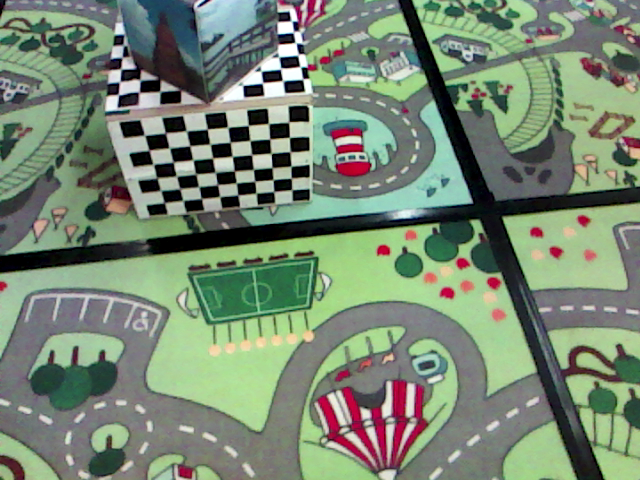
\includegraphics[width=70mm]{misc/16-6_too-low.png}
  \caption{Typical image with circle trajectory height and radius both set to 1.2m}
  \label{f: too low}
\end{figure}

\begin{figure}[h]
  \centering
    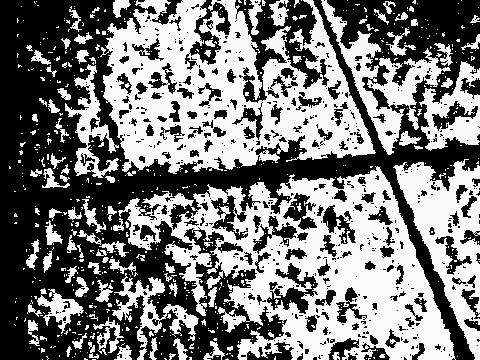
\includegraphics[width=70mm]{misc/16-6_too-low_depth.png}
  \caption{Depth image corresponding to Figure \ref{f: too low}}
  \label{f: too low depth}
\end{figure}


\section{Stuff to do}
\begin{itemize}
\item Fix quadcopter
\item Adjust quadcopter trajectory so that it can see the top box
\item Investigate data
\begin{itemize}
\item \sout{Investigate boxes to determine which ones can be picked up as point clouds}
\end{itemize}
\item Investigate registration algorithm
\begin{itemize}
\item Generate 3D object in MATLAB that I can get points from from various camera poses (may also need to get RGB and depth images if we're going with that approach?)
\item Apply registration algorithm to generated point clouds (ground truth known) -- without noise first, then add noise. Get error in true and estimated translation and rotation.
\end{itemize}
\item Reading
\begin{itemize}
\item Incorporating RGB and depth images -- feature matching
\end{itemize}
\end{itemize}

\end{document}